\section{Performance and Validation}

\subsection{Performance and Scaling}
We perform weak scaling tests for simulations of convection preceding ignition in a spherical, full-star sub-Chandrasekhar mass white dwarf.
The simulation setup remains the same as reported in Section 3 of \cite{MAESTRO_AMR} and originally used in \cite{MAESTRO_convection}, and thus we emphasize that these scaling tests are performed using meaningful, scientific calculations.
Here, we perform simulations using $256^3, 512^3, 768^3, 1024^3, 1280^3$, and $1536^3$ grid cells on a spatially uniform grid (no AMR).
We divide each simulation into $64^3$ grids, so this simulations contain between 64 grids ($256^3$) and 13,824 grids ($1536^3$).
These simulations were performed using the NERSC cori system on the Intel Xeon Phi (KNL) partition.
Each node contains 68 cores, each capable of supporting up to 4 hardware threads (i.e., a maximum of 272 hardware threads per node).
For these tests, we assign 4 MPI tasks to each node, and 16 OpenMP threads per MPI process.
For $64^3$ grids we discovered that using more than 16 OpenMP threads did not decrease the wallclock time due to a lack of work available per grid; in principle one could use larger grids, fewer MPI processes, and more threads per MPI process, however the overall wallclock time would increase except for extremely large numbers of MPI processes (beyond the range we tested here).


In Figure \ref{fig:scaling} we compare the wallclock time per time step for the original BoxLib-based MAESTRO implementation to the AMReX MAESTReX implementation with the same algorithm.
We also include a plot of MAESTROeX without base state evolution.





The y-axis is the wallclock time per time step, and the x-axis represents total core count (in this case, the total number of OpenMP threads).

We split each KNL node to contain 4 MPI processes with 16 threads each.  We note that KNL can support up to 272 hardware threads per node (i.e., 68 hardware threads per MPI process since here we assign 4 MPI processes per node), but testing reveals that using $64^3$ grids, additional threads do not decrease the wallclock time.  Thus, the more accurate measure of weak scaling is to consider the number of MPI processes, since the scaling plot would look virtually identical for larger thread counts.


In principle, we could use larger grids and use more OpenMP threads per MPI process, but the overall wallclock time would increase.

The computational domain for each simulation is divided into $64^3$ grid cells, and we assign 1 MPI process to each grid.
We used simulations ranging from $256^3$ grid cells (64 MPI processes, corresponding to 1024 total threads) up to $1536^3$ grid cells (13,824 MPI processes, corresponding to 221,184 total threads).
Note that the largest simulation used roughly 36\% of the entire computational system.
We see that the total increas in wallclock time from the smallest to largest simulation is roughly 41\%, which is quite remarkable given that there are 3 linear solves per time step.

Include a plot showing the linear solver scaling, and a discussion about how the bottleneck for typical MAESTRO simulations is the averaging operator.

\MarginPar{Include commentary about new temporal algorithm, and new temporal algorithm with irregular base state}
For the new temporal algorithm, and the option for irregular base state mapping, <COMMENT HERE ABOUT RUNTIME>

%%%%%%%%%%%%%%%%%%%%%%%%%%%%%
\begin{figure}[htb]
\begin{center}
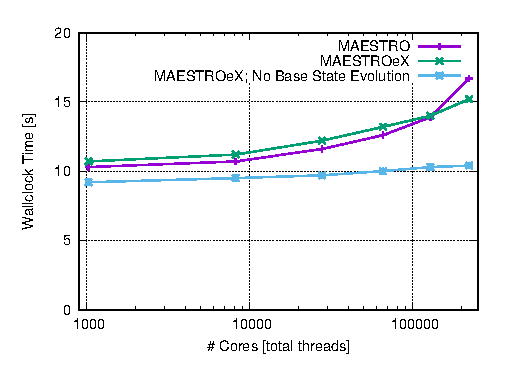
\includegraphics[width=2.75in]{./figs/MAESTRO_scaling1}
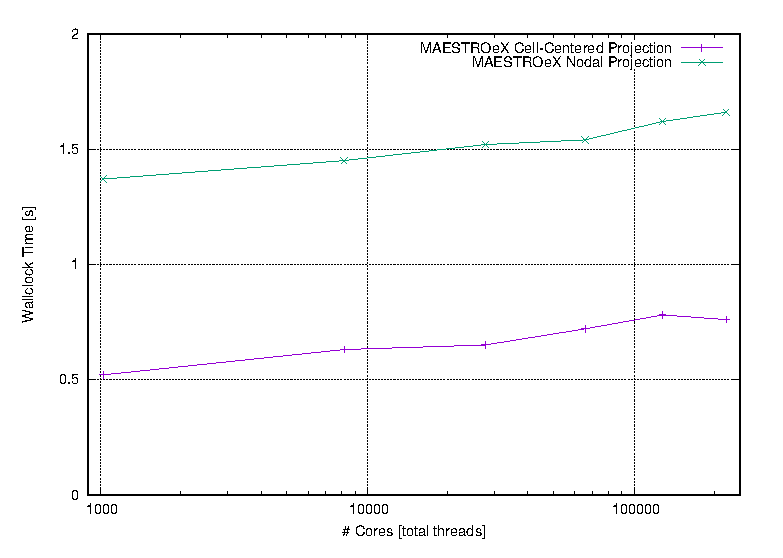
\includegraphics[width=2.75in]{./figs/MAESTRO_scaling2}
\caption{\label{fig:scaling} (Left) Weak scaling results for a spherical, full-star sub-Chandrasekhar mass white dwarf calculation using the original MAESTRO code, MAESTROeX, and MAESTROeX with base state evolution disabled.  Shown is the average wallclock time per time step.
(Right) Weak scaling results showing the average wallclock time per time step spent in the cell-centered and nodal linear solvers within a full time step of the aforementioned simulations.}
\end{center}
\end{figure}
%%%%%%%%%%%%%%%%%%%%%%%%%%%%%


\subsection{AMR Performance}
Show 3D reacting bubble rise performance.
Show 3-level spherical performance (stats won't be as good but explain why: refining a larger percentage of grid)
Images of grid configuration.

\subsection{White Dwarf Convection}
white dwarf convection runs with 3 algorithms (original, new temporal, new temporal + irregular base state)

Show 3-level wdconvect
